\documentclass[a4paper, 11pt]{article}
\usepackage{comment} % enables the use of multi-line comments (\ifx \fi) 
\usepackage{lipsum} %This package just generates Lorem Ipsum filler text. 
\usepackage{fullpage} % changes the margin
\usepackage[spanish]{babel}
\usepackage[utf8]{inputenc}
\usepackage{graphicx}


\usepackage{circuitikz}
\usepackage{tikz}
%\usepackage[utf8]{inputenc} %Indica qué codificación se está usando ISO-8859-1(latin1)  o utf8  
\usepackage{amsmath} % Comandos extras para matemáticas (cajas para ecuaciones,
% etc)
%\usepackage{subfig}
\usepackage{amssymb} % Símbolos matemáticos (por lo tanto)
\usepackage{graphicx} % Incluir imágenes en LaTeX
\usepackage{subfloat}
\usepackage{booktabs} % tablas
\usepackage{color} % Para colorear texto
\usepackage{subfigure} % subfiguras
\usepackage{float} %Podemos usar el especificador [H] en las figuras para que se
% queden donde queramos     
\usepackage{capt-of}  % Permite usar etiquetas fuera de elementos flotantes
% (etiquetas de figuras)
\usepackage{sidecap} % Para poner el texto de las imágenes al lado
	\sidecaptionvpos{figure}{c} % Para que el texto se alinie al centro vertical
\usepackage{caption} % Para poder quitar numeracion de figuras
\usepackage{amsmath}
% etc (\od, \dif, etc)

 
\usepackage{anysize} 
\begin{document}
%Header-Make sure you update this information!!!!
\noindent
\large\textbf{Tarea} \hfill \textbf{José Ricardo Soro Jara} \\
\normalsize Dispositivos Semiconductores \hfill  \\ \textbf{B36853}
\hfill Fecha: 15/10/2018 \\

\section*{Valores por defecto}
A la hora de simular los valores por defecto se tuvo resultados muy satisfactorios donde se tuvo que modificar el valor del w hasta obtener resultados congruentes con lo esperado y se obtuvo el siguiente resultado:
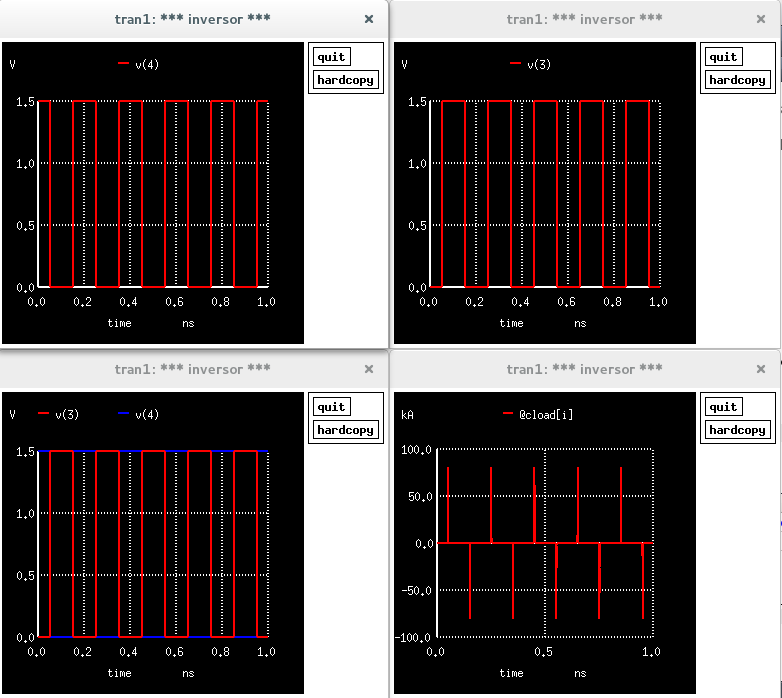
\includegraphics[scale=0.420]{def.png}

\section*{Valores típicos}
No se logro hacer funcionar con modelos reales; se vario todo lo que se pudo el Width del canal pero no se consiguió en ninguno de los modos el comportamiento buscado

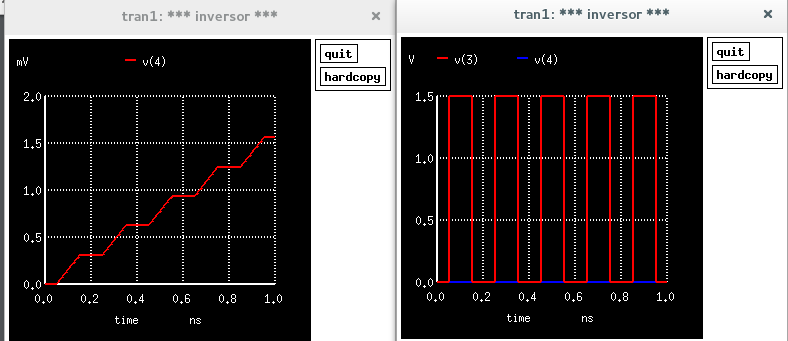
\includegraphics[scale=0.420]{typReal.png}

\section*{Valores mínimos}
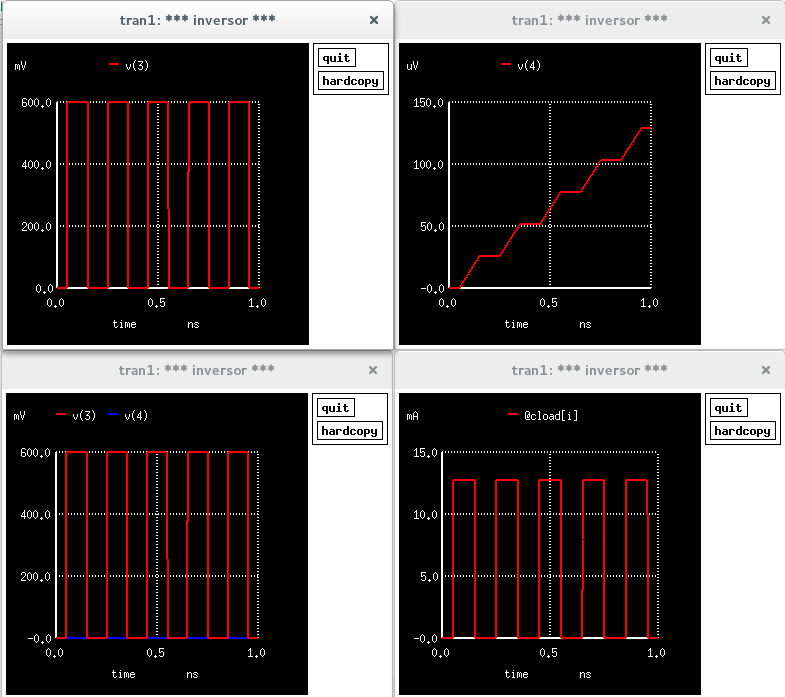
\includegraphics[scale=0.420]{min.png}


\section*{Valores máximos}
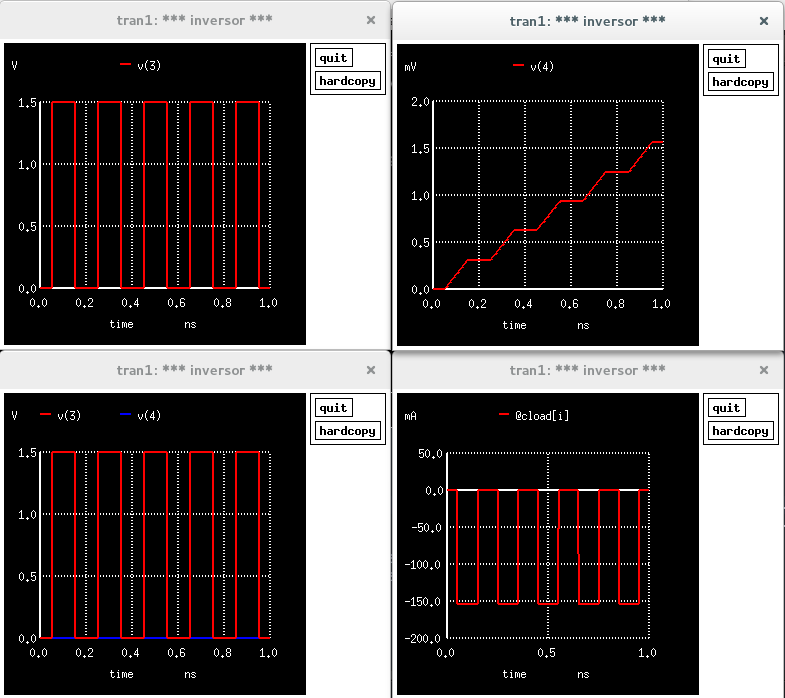
\includegraphics[scale=0.420]{max.png}


\end{document}
